%% GENERATED by tools/from_docs.py from stepss-docs. Do not edit by hand:
%% edit the page named below in stepss-docs and regenerate.
%% source: stepss-docs/src/content/docs/models/synchronous-machine.md

\chapter{Synchronous machine models}\label{doc:model-sync}

This page documents the mathematical model of the synchronous machine implemented in RAMSES. The model is a detailed sixth-order model, including four rotor windings with saturation effects. It uses the Equal-Mutual-Flux-Linkage (EMFL) per unit system and supports detailed (round rotor, salient-pole) and simplified (field winding only) configurations through model switches.

\begin{center}\rule{0.5\linewidth}{0.5pt}\end{center}

\section{Model Switches}\label{model-sync:model-switches}

To accommodate different rotor configurations within a single model, integer ``model switches'' are defined:

{\def\LTcaptype{none} % do not increment counter
\begin{small}\begin{longtable}[]{@{}ll@{}}
\toprule\noalign{}
Switch & Meaning \\
\midrule\noalign{}
\endhead
\bottomrule\noalign{}
\endlastfoot
\(S_{d1}\) & 1 if there is a damper winding \(d1\), 0 otherwise \\
\(S_{q1}\) & 1 if there is a damper winding \(q1\), 0 otherwise \\
\(S_{q2}\) & 1 if there is an equivalent winding \(q2\), 0 otherwise \\
\end{longtable}\end{small}
}

{\def\LTcaptype{none} % do not increment counter
\begin{small}\begin{longtable}[]{@{}
  >{\raggedright\arraybackslash}p{(\linewidth - 2\tabcolsep) * \real{0.4118}}
  >{\raggedright\arraybackslash}p{(\linewidth - 2\tabcolsep) * \real{0.5882}}@{}}
\toprule\noalign{}
\begin{minipage}[b]{\linewidth}\raggedright
Model
\end{minipage} & \begin{minipage}[b]{\linewidth}\raggedright
Switches
\end{minipage} \\
\midrule\noalign{}
\endhead
\bottomrule\noalign{}
\endlastfoot
Detailed, round rotor & \(S_{d1} = 1,\; S_{q1} = 1,\; S_{q2} = 1\) \\
Detailed, salient-pole rotor & \(S_{d1} = 1,\; S_{q1} = 1,\; S_{q2} = 0\) \\
Detailed, salient-pole rotor & \(S_{d1} = 1,\; S_{q1} = 0,\; S_{q2} = 1\) \\
Simplified, field winding only & \(S_{d1} = 0,\; S_{q1} = 0,\; S_{q2} = 0\) \\
\end{longtable}\end{small}
}

The second and third combinations yield the same results. Models with fewer rotor windings are specified by skipping the corresponding data in the \texttt{SYNC\_MACH} record (see \hyperref[model-sync:omitting-rotor-circuits]{below}).

\begin{center}\rule{0.5\linewidth}{0.5pt}\end{center}

\section{Park Transformation}\label{model-sync:park-transformation}

The well-known Park transformation is used to replace time-varying inductances and oscillatory stator currents and voltages with constant values. The machine is represented by equivalent windings along the direct (\(d\)) and quadrature (\(q\)) axes: a field winding \(f\) and damper winding \(d1\) on the \(d\) axis, and windings \(q1\), \(q2\) on the \(q\) axis:

\begin{figure}[htbp]
\centering
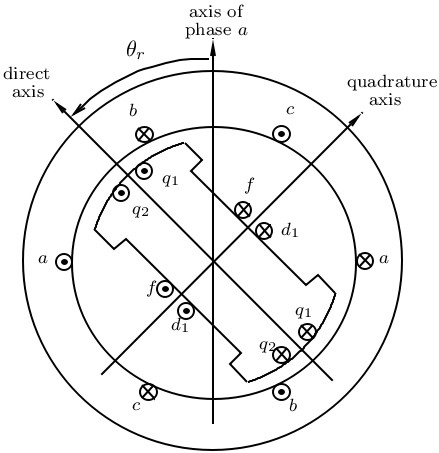
\includegraphics[width=0.42\linewidth]{figures/sync-windings}
\caption{Synchronous machine windings}
\end{figure}

\begin{figure}[htbp]
\centering
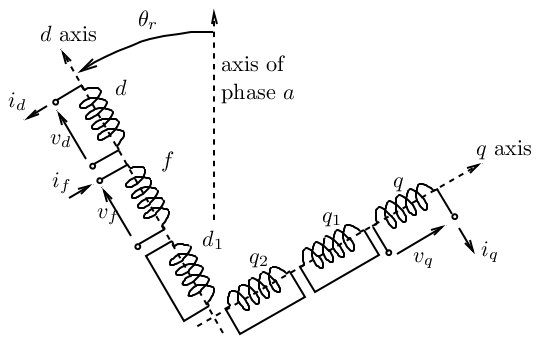
\includegraphics[width=0.50\linewidth]{figures/sync-park}
\caption{Equivalent windings of the Park transformation}
\end{figure}

\begin{center}\rule{0.5\linewidth}{0.5pt}\end{center}

\section{Flux-Current Relationships}\label{model-sync:flux-current-relationships}

Using the EMFL per unit system, the relationship between magnetic flux linkages and currents is:

\[
\begin{pmatrix} \psi_d \\ \psi_f \\ \psi_{d1} \end{pmatrix} = \begin{pmatrix} L_\ell + M_d & M_d & S_{d1} M_d \\ M_d & L_{\ell f} + M_d & S_{d1} M_d \\ S_{d1} M_d & S_{d1} M_d & L_{\ell d1} + S_{d1} M_d \end{pmatrix} \begin{pmatrix} i_d \\ i_f \\ i_{d1} \end{pmatrix}
\]

\[
\begin{pmatrix} \psi_q \\ \psi_{q1} \\ \psi_{q2} \end{pmatrix} = \begin{pmatrix} L_\ell + M_q & S_{q1} M_q & S_{q2} M_q \\ S_{q1} M_q & L_{\ell q1} + S_{q1} M_q & S_{q2} M_q \\ S_{q2} M_q & S_{q2} M_q & L_{\ell q2} + S_{q2} M_q \end{pmatrix} \begin{pmatrix} i_q \\ i_{q1} \\ i_{q2} \end{pmatrix}
\]

The \(d\) and \(q\) components of the air-gap flux are:

\[
\psi_{ad} = M_d(i_d + i_f + S_{d1} i_{d1})
\]

\[
\psi_{aq} = M_q(i_q + S_{q1} i_{q1} + S_{q2} i_{q2})
\]

Individual flux linkages in terms of air-gap flux:

\[
\psi_d = L_\ell i_d + \psi_{ad}
\]

\[
\psi_f = L_{\ell f} i_f + \psi_{ad}
\]

\[
\psi_{d1} = L_{\ell d1} i_{d1} + S_{d1} \psi_{ad}
\]

\[
\psi_q = L_\ell i_q + \psi_{aq}
\]

\[
\psi_{q1} = L_{\ell q1} i_{q1} + S_{q1} \psi_{aq}
\]

\[
\psi_{q2} = L_{\ell q2} i_{q2} + S_{q2} \psi_{aq}
\]

Rotor currents from flux linkages:

\[
i_f = \frac{\psi_f - \psi_{ad}}{L_{\ell f}}, \qquad i_{d1} = \frac{\psi_{d1} - S_{d1} \psi_{ad}}{L_{\ell d1}}, \qquad i_{q1} = \frac{\psi_{q1} - S_{q1} \psi_{aq}}{L_{\ell q1}}, \qquad i_{q2} = \frac{\psi_{q2} - S_{q2} \psi_{aq}}{L_{\ell q2}}
\]

\begin{center}\rule{0.5\linewidth}{0.5pt}\end{center}

\section{Saturation Model}\label{model-sync:saturation-model}

Let \(M_d^u\) and \(M_q^u\) be the unsaturated direct- and quadrature-axis mutual inductances. The saturated values \(M_d\) and \(M_q\) are:

\[
M_d = \frac{M_d^u}{1 + m \left(\sqrt{\psi_{ad}^2 + \psi_{aq}^2}\right)^n}
\]

\[
M_q = \frac{M_q^u}{1 + m \left(\sqrt{\psi_{ad}^2 + \psi_{aq}^2}\right)^n}
\]

where \(m\) and \(n\) are the saturation exponents specified in the \texttt{SYNC\_MACH} record.

Substituting into the air-gap flux expressions yields the algebraic equations:

\[
\psi_{ad} \left( \frac{1 + m(\sqrt{\psi_{ad}^2 + \psi_{aq}^2})^n}{M_d^u} + \frac{1}{L_{\ell f}} + \frac{S_{d1}}{L_{\ell d1}} \right) - i_d - \frac{1}{L_{\ell f}} \psi_f - \frac{S_{d1}}{L_{\ell d1}} \psi_{d1} = 0
\]

\[
\psi_{aq} \left( \frac{1 + m(\sqrt{\psi_{ad}^2 + \psi_{aq}^2})^n}{M_q^u} + \frac{S_{q1}}{L_{\ell q1}} + \frac{S_{q2}}{L_{\ell q2}} \right) - i_q - \frac{S_{q1}}{L_{\ell q1}} \psi_{q1} - \frac{S_{q2}}{L_{\ell q2}} \psi_{q2} = 0
\]

\begin{center}\rule{0.5\linewidth}{0.5pt}\end{center}

\section{Reference Frame}\label{model-sync:reference-frame}

All synchronous machines have their rotor positions referred to the \(x\) axis of the network reference frame (see \hyperref[ch-refinit]{Reference Frames \& Initialization}). The \textbf{rotor angle} \(\delta\) of a machine is the angle difference between its \(q\) axis and the \(x\) reference axis. In steady state, the machine internal emf (proportional to field current) is aligned along the \(q\) axis; \(\delta\) is thus the phase angle of that emf with respect to the \(x\) axis.

\begin{figure}[htbp]
\centering
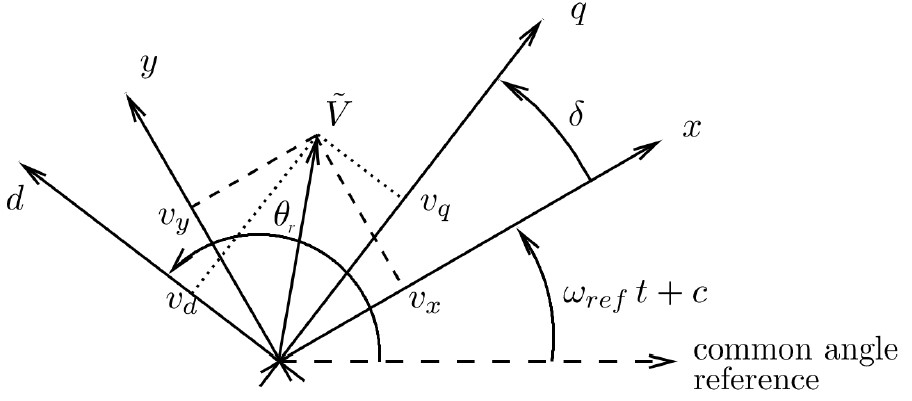
\includegraphics[width=0.65\linewidth]{figures/sync-delta}
\caption{Definition of the rotor angle delta}
\end{figure}

The \(d\) and \(q\) components of the stator voltage and current relate to the network \((x, y)\) components through the rotor angle \(\delta\):

\[
\begin{pmatrix} v_d \\ v_q \end{pmatrix} = \begin{pmatrix} -\sin\delta & \cos\delta \\ \cos\delta & \sin\delta \end{pmatrix} \begin{pmatrix} v_x \\ v_y \end{pmatrix}
\]

\[
\begin{pmatrix} i_d \\ i_q \end{pmatrix} = \begin{pmatrix} -\sin\delta & \cos\delta \\ \cos\delta & \sin\delta \end{pmatrix} \begin{pmatrix} i_x \\ i_y \end{pmatrix}
\]

After transformation, the air-gap flux algebraic equations in \((x, y)\) coordinates become:

\[
\psi_{ad} \left( \frac{1 + m(\sqrt{\psi_{ad}^2 + \psi_{aq}^2})^n}{M_d^u} + \frac{1}{L_{\ell f}} + \frac{S_{d1}}{L_{\ell d1}} \right) + \sin\delta\, i_x - \cos\delta\, i_y - \frac{1}{L_{\ell f}} \psi_f - \frac{S_{d1}}{L_{\ell d1}} \psi_{d1} = 0
\]

\[
\psi_{aq} \left( \frac{1 + m(\sqrt{\psi_{ad}^2 + \psi_{aq}^2})^n}{M_q^u} + \frac{S_{q1}}{L_{\ell q1}} + \frac{S_{q2}}{L_{\ell q2}} \right) - \cos\delta\, i_x - \sin\delta\, i_y - \frac{S_{q1}}{L_{\ell q1}} \psi_{q1} - \frac{S_{q2}}{L_{\ell q2}} \psi_{q2} = 0
\]

\begin{center}\rule{0.5\linewidth}{0.5pt}\end{center}

\section{Park Equations}\label{model-sync:park-equations}

\subsection{Original form}\label{model-sync:original-form}

\[
v_d = -R_a i_d - \omega \psi_q \qquad\qquad v_q = -R_a i_q + \omega \psi_d
\]

\[
\frac{d\psi_f}{dt} = \omega_N (K_f v_f - R_f i_f) \qquad
\frac{d\psi_{d1}}{dt} = -\omega_N R_{d1} i_{d1} \qquad
\frac{d\psi_{q1}}{dt} = -\omega_N R_{q1} i_{q1} \qquad
\frac{d\psi_{q2}}{dt} = -\omega_N R_{q2} i_{q2}
\]

where \(R_a\) is the stator (armature) resistance, \(R_f\) the field winding resistance, \(R_{d1}\), \(R_{q1}\), \(R_{q2}\) the rotor winding resistances, \(\omega\) the rotor speed (pu), \(\omega_N = 2\pi f_{nom}\) the nominal angular frequency (rad/s), \(v_f\) the field voltage, and \(K_f\) a coefficient to pass from per unit values of the excitation system to per unit values of the machine.

The stator equations are transformed to the \((x, y)\) frame using the rotation matrices above, and the rotor currents are eliminated using the flux-current relationships, yielding the equations actually solved by RAMSES:

\subsection{\texorpdfstring{Stator equations (algebraic, in \(x\)-\(y\) frame)}{Stator equations (algebraic, in x-y frame)}}\label{model-sync:stator-equations-algebraic-in-x-y-frame}

\[
0 = \sin\delta\, v_x - \cos\delta\, v_y + (R_a \sin\delta - \omega L_\ell \cos\delta)\, i_x - (R_a \cos\delta + \omega L_\ell \sin\delta)\, i_y - \omega \psi_{aq}
\]

\[
0 = -\cos\delta\, v_x - \sin\delta\, v_y - (R_a \cos\delta + \omega L_\ell \sin\delta)\, i_x - (R_a \sin\delta - \omega L_\ell \cos\delta)\, i_y + \omega \psi_{ad}
\]

\subsection{Rotor equations (differential)}\label{model-sync:rotor-equations-differential}

\[
\frac{d\psi_f}{dt} = \omega_N \left( K_f v_f - R_f \frac{\psi_f - \psi_{ad}}{L_{\ell f}} \right)
\]

\[
\frac{d\psi_{d1}}{dt} = -\omega_N R_{d1} \frac{\psi_{d1} - S_{d1} \psi_{ad}}{L_{\ell d1}}
\]

\[
\frac{d\psi_{q1}}{dt} = -\omega_N R_{q1} \frac{\psi_{q1} - S_{q1} \psi_{aq}}{L_{\ell q1}}
\]

\[
\frac{d\psi_{q2}}{dt} = -\omega_N R_{q2} \frac{\psi_{q2} - S_{q2} \psi_{aq}}{L_{\ell q2}}
\]

\begin{center}\rule{0.5\linewidth}{0.5pt}\end{center}

\section{Rotor Motion}\label{model-sync:rotor-motion}

\[
\frac{1}{\omega_N} \frac{d\delta}{dt} = \omega - \omega_{ref}
\]

\[
2H \frac{d\omega}{dt} = K_m T_m - T_e - D(\omega - \omega_{ref})
\]

where \(H\) is the inertia constant (in s), \(T_m\) the mechanical torque produced by the turbine, \(K_m\) a coefficient to pass from per unit values of the turbine to per unit values of the machine, and \(\omega_{ref}\) the angular speed of the reference axes: \(\omega_{coi}\) in the COI reference frame, or 1 pu in the synchronous frame (selected by the \texttt{\$OMEGA\_REF} solver setting).

The electromagnetic torque \(T_e\) is:

\[
T_e = \psi_{ad} i_q - \psi_{aq} i_d = \psi_{ad}(\cos\delta\, i_x + \sin\delta\, i_y) - \psi_{aq}(-\sin\delta\, i_x + \cos\delta\, i_y)
\]

\begin{center}\rule{0.5\linewidth}{0.5pt}\end{center}

\section{State Variables and Equations Summary}\label{model-sync:state-variables-and-equations-summary}

The model has \textbf{10 state variables}: \(i_x\), \(i_y\), \(\psi_{ad}\), \(\psi_{aq}\), \(\psi_f\), \(\psi_{d1}\), \(\psi_{q1}\), \(\psi_{q2}\), \(\delta\), \(\omega\).

These are balanced by:
- \textbf{4 algebraic equations}: air-gap flux (d and q), stator voltage (d and q)
- \textbf{6 differential equations}: field flux, d1 damper flux, q1 damper flux, q2 damper flux, rotor angle, rotor speed

\begin{center}\rule{0.5\linewidth}{0.5pt}\end{center}

\section{Per Unit System and IBRATIO}\label{model-sync:per-unit-system-and-ibratio}

The synchronous machine model uses the EMFL per unit system, while the excitation system typically uses its own per unit system. The parameter \texttt{IBRATIO} bridges these two bases:

\[
IBRATIO = \frac{I_{fB}^{mac}}{I_{fB}^{exc}}
\]

where \(I_{fB}^{mac}\) is the field winding base current in the machine model and \(I_{fB}^{exc}\) is the base current in the excitation system model. The relationship between per-unit field currents in the two systems is:

\[
IBRATIO = \frac{i_{f,pu}^{exc}}{i_{f,pu}^{mac}}
\]

\subsection{Common per unit conventions for IBRATIO}\label{model-sync:common-per-unit-conventions-for-ibratio}

\textbf{Open-circuit unsaturated machine} (most common): \(I_{fB}^{exc}\) is the field current that produces nominal stator voltage (\(V = 1\) pu) at nominal speed (\(\omega = 1\) pu) with the stator open, neglecting saturation:

\[
IBRATIO = M_d^u = X_d^u - X_\ell
\]

\textbf{Open-circuit saturated machine}: Same conditions but with saturation:

\[
IBRATIO = \frac{M_d^u}{1 + m} = \frac{X_d^u - X_\ell}{1 + m}
\]

\textbf{Saturated machine at nominal operating conditions}: \(I_{fB}^{exc}\) is the field current when the machine produces nominal active and reactive powers (\(P = \cos\phi_N\), \(Q = \sin\phi_N\)) at nominal voltage and speed, with saturation.

\begin{center}\rule{0.5\linewidth}{0.5pt}\end{center}

\section{SYNC\_MACH Record}\label{model-sync:sync_mach-record}

The machine model requires the nominal system frequency, given by the \textbf{mandatory} \texttt{FNOM} record (see \hyperref[ch-settings]{Solver Settings}):

\begin{Verbatim}
FNOM F ;
\end{Verbatim}

where \texttt{F} is the nominal frequency in Hz.

The synchronous machine itself is declared with the \texttt{SYNC\_MACH} record:

\begin{Verbatim}
SYNC_MACH name bus FP FQ P Q SNOM Pnom H D IBRATIO
          TYPE_MOD  <14 machine parameters, see below>
          EXC exc_type param1 param2 ...
          TOR tor_type param1 param2 ... ;
\end{Verbatim}

\texttt{TYPE\_MOD} is a keyword selecting which of two \textbf{equivalent parameter formats}
the 14 machine parameters that follow are given in:

\begin{itemize}
\item
  \textbf{\texttt{RL}}: the inductances and resistances of the Park model are supplied
  directly:

\begin{Verbatim}
RL  Ll Mdu Llf Lld1 Mqu Llq1 Llq2 m n Ra Rf Rd1 Rq1 Rq2
\end{Verbatim}
\item
  \textbf{\texttt{XT}}: characteristic reactances and open-circuit time constants are
  supplied; RAMSES converts them internally to the Park parameters (see
  \hyperref[doc:model-sync-conv]{Parameter Conversion}):

\begin{Verbatim}
XT  Xl Xd X'd X"d Xq X'q X"q m n Ra T'do T"do T'qo T"qo
\end{Verbatim}
\end{itemize}

\subsection{Common parameters}\label{model-sync:common-parameters}

{\def\LTcaptype{none} % do not increment counter
\begin{small}\begin{longtable}[]{@{}
  >{\raggedright\arraybackslash}p{(\linewidth - 4\tabcolsep) * \real{0.3667}}
  >{\raggedright\arraybackslash}p{(\linewidth - 4\tabcolsep) * \real{0.4333}}
  >{\raggedright\arraybackslash}p{(\linewidth - 4\tabcolsep) * \real{0.2000}}@{}}
\toprule\noalign{}
\begin{minipage}[b]{\linewidth}\raggedright
Parameter
\end{minipage} & \begin{minipage}[b]{\linewidth}\raggedright
Description
\end{minipage} & \begin{minipage}[b]{\linewidth}\raggedright
Unit
\end{minipage} \\
\midrule\noalign{}
\endhead
\bottomrule\noalign{}
\endlastfoot
\texttt{name} & Machine name (max 20 characters) & \\
\texttt{bus} & Connection bus name (max 8 characters) & \\
\texttt{FP} & Active power participation fraction (0--1) & \\
\texttt{FQ} & Reactive power participation fraction (0--1) & \\
\texttt{P} & Initial active power (used when FP = 0) & MW \\
\texttt{Q} & Initial reactive power (used when FQ = 0) & Mvar \\
\texttt{SNOM} & Nominal apparent power, used as base power in the machine model & MVA \\
\texttt{Pnom} & Nominal active power of the turbine, used as base power for the turbine model & MW \\
\texttt{H} & Inertia constant & s \\
\texttt{D} & Damping coefficient (usually set to zero when the damper windings are modelled) & pu \\
\texttt{IBRATIO} & Field current base ratio \(I_{fB}^{mac}/I_{fB}^{exc}\) (see above) & pu \\
\texttt{TYPE\_MOD} & Parameter format keyword: \texttt{RL} or \texttt{XT} (case-insensitive) & \\
\end{longtable}\end{small}
}

\subsection{\texorpdfstring{Machine parameters, \texttt{XT} format}{Machine parameters, XT format}}\label{model-sync:machine-parameters-xt-format}

{\def\LTcaptype{none} % do not increment counter
\begin{small}\begin{longtable}[]{@{}
  >{\raggedright\arraybackslash}p{(\linewidth - 4\tabcolsep) * \real{0.3667}}
  >{\raggedright\arraybackslash}p{(\linewidth - 4\tabcolsep) * \real{0.4333}}
  >{\raggedright\arraybackslash}p{(\linewidth - 4\tabcolsep) * \real{0.2000}}@{}}
\toprule\noalign{}
\begin{minipage}[b]{\linewidth}\raggedright
Parameter
\end{minipage} & \begin{minipage}[b]{\linewidth}\raggedright
Description
\end{minipage} & \begin{minipage}[b]{\linewidth}\raggedright
Unit
\end{minipage} \\
\midrule\noalign{}
\endhead
\bottomrule\noalign{}
\endlastfoot
\texttt{Xl} & Leakage reactance \(L_\ell\) & pu \\
\texttt{Xd} & d-axis synchronous reactance (\(M_d^u = X_d - X_\ell\)) & pu \\
\texttt{X\textquotesingle{}d} & d-axis transient reactance (must be smaller than \texttt{Xd}) & pu \\
\texttt{X"d} & d-axis subtransient reactance (\texttt{*} if no \(d1\) damper winding) & pu \\
\texttt{Xq} & q-axis synchronous reactance (\(M_q^u = X_q - X_\ell\)) & pu \\
\texttt{X\textquotesingle{}q} & q-axis transient reactance (\texttt{*} if no \(q1\) winding; must be smaller than \texttt{Xq}) & pu \\
\texttt{X"q} & q-axis subtransient reactance (\texttt{*} if no \(q2\) winding) & pu \\
\texttt{m} & Saturation coefficient (set to 0 to neglect saturation) & \\
\texttt{n} & Saturation exponent (ignored when \texttt{m} = 0) & \\
\texttt{Ra} & Armature resistance & pu \\
\texttt{T\textquotesingle{}do} & d-axis open-circuit transient time constant & s \\
\texttt{T"do} & d-axis open-circuit subtransient time constant (\texttt{*} if no \(d1\) damper winding) & s \\
\texttt{T\textquotesingle{}qo} & q-axis open-circuit transient time constant (\texttt{*} if no \(q1\) winding) & s \\
\texttt{T"qo} & q-axis open-circuit subtransient time constant (\texttt{*} if no \(q2\) winding) & s \\
\end{longtable}\end{small}
}

\subsection{\texorpdfstring{Machine parameters, \texttt{RL} format}{Machine parameters, RL format}}\label{model-sync:machine-parameters-rl-format}

{\def\LTcaptype{none} % do not increment counter
\begin{small}\begin{longtable}[]{@{}
  >{\raggedright\arraybackslash}p{(\linewidth - 4\tabcolsep) * \real{0.3667}}
  >{\raggedright\arraybackslash}p{(\linewidth - 4\tabcolsep) * \real{0.4333}}
  >{\raggedright\arraybackslash}p{(\linewidth - 4\tabcolsep) * \real{0.2000}}@{}}
\toprule\noalign{}
\begin{minipage}[b]{\linewidth}\raggedright
Parameter
\end{minipage} & \begin{minipage}[b]{\linewidth}\raggedright
Description
\end{minipage} & \begin{minipage}[b]{\linewidth}\raggedright
Unit
\end{minipage} \\
\midrule\noalign{}
\endhead
\bottomrule\noalign{}
\endlastfoot
\texttt{Ll} & Stator leakage inductance \(L_\ell\) & pu \\
\texttt{Mdu} & Unsaturated d-axis mutual inductance \(M_d^u\) & pu \\
\texttt{Llf} & Field winding leakage inductance \(L_{\ell f}\) & pu \\
\texttt{Lld1} & \(d1\) damper leakage inductance \(L_{\ell d1}\) (\texttt{*} if no \(d1\) winding) & pu \\
\texttt{Mqu} & Unsaturated q-axis mutual inductance \(M_q^u\) & pu \\
\texttt{Llq1} & \(q1\) winding leakage inductance \(L_{\ell q1}\) (\texttt{*} if no \(q1\) winding) & pu \\
\texttt{Llq2} & \(q2\) winding leakage inductance \(L_{\ell q2}\) (\texttt{*} if no \(q2\) winding) & pu \\
\texttt{m} & Saturation coefficient (set to 0 to neglect saturation) & \\
\texttt{n} & Saturation exponent (ignored when \texttt{m} = 0) & \\
\texttt{Ra} & Armature resistance & pu \\
\texttt{Rf} & Field winding resistance \(R_f\) & pu \\
\texttt{Rd1} & \(d1\) damper resistance \(R_{d1}\) (\texttt{*} if no \(d1\) winding) & pu \\
\texttt{Rq1} & \(q1\) winding resistance \(R_{q1}\) (\texttt{*} if no \(q1\) winding) & pu \\
\texttt{Rq2} & \(q2\) winding resistance \(R_{q2}\) (\texttt{*} if no \(q2\) winding) & pu \\
\end{longtable}\end{small}
}

\subsection{Omitting rotor circuits}\label{model-sync:omitting-rotor-circuits}

A rotor circuit the machine does not have is skipped by putting \texttt{*} in \textbf{both}
of its fields, the inductance/reactance \textbf{and} the matching
resistance/time-constant field (specifying only one is an error):

{\def\LTcaptype{none} % do not increment counter
\begin{small}\begin{longtable}[]{@{}llll@{}}
\toprule\noalign{}
Circuit & \texttt{RL} fields & \texttt{XT} fields & Model switch set to 0 \\
\midrule\noalign{}
\endhead
\bottomrule\noalign{}
\endlastfoot
\(d1\) damper & \texttt{Lld1}, \texttt{Rd1} & \texttt{X"d}, \texttt{T"do} & \(S_{d1}\) \\
\(q1\) winding & \texttt{Llq1}, \texttt{Rq1} & \texttt{X\textquotesingle{}q}, \texttt{T\textquotesingle{}qo} & \(S_{q1}\) \\
\(q2\) winding & \texttt{Llq2}, \texttt{Rq2} & \texttt{X"q}, \texttt{T"qo} & \(S_{q2}\) \\
\end{longtable}\end{small}
}

The combination \(S_{d1} = 0\) with \(S_{q1} = S_{q2} = 1\) (field winding plus
both q-axis windings but no d-axis damper) is rejected. In the \texttt{XT} format,
if the fitted Park parameters come out negative, RAMSES logs an
``unrealistic Park inductances or resistances'' warning: the supplied
reactances and time constants are physically inconsistent.

All reactances, inductances and resistances are in per unit on the machine base
(\(S_{nom}\), nominal voltage), using the EMFL per unit system for the rotor
quantities. Time constants are entered in seconds and normalised internally by
\(t_b = 1/(2\pi f_{nom})\).

The \texttt{EXC} and \texttt{TOR} sub-records specify the excitation system and turbine-governor models. See the \hyperref[doc:model-index]{Model Reference} for available models.

\begin{docsnote}{Note}

The FP, FQ, P, Q fields control how the machine's initial operating point is determined from the power flow solution. See \hyperref[ch-refinit]{Reference Frames \& Initialization} for details.

\end{docsnote}

\begin{center}\rule{0.5\linewidth}{0.5pt}\end{center}

\section{Initialization Output}\label{model-sync:initialization-output}

At initialization RAMSES prints one block per synchronous machine. Example:

\begin{Verbatim}
NUMBER OF SYNCHRONOUS MACHINES :    1

machine              at bus                 V            P           Q        delta    sat    island  br
                     excit model          vf(pu)   torque model               Tm(pu)

G5                   5                    1.0000    450.00186     68.49769    70.99   1.0000       1    1
                     exc_GENERIC          2.3680   THERMAL_GENERIC1          0.97826
\end{Verbatim}

Here the machine G5, connected to bus 5, is in service (\texttt{br\ =\ 1}) and injects about 450 MW and 68 Mvar into the grid under a bus voltage of 1 pu.

\begin{itemize}
\tightlist
\item
  \texttt{delta} is the initial value of the rotor angle \(\delta\), in \textbf{degrees}.
\item
  \texttt{sat} is the saturation factor
  \[
  sat = 1 + m \left( \sqrt{\psi_{ad}^2 + \psi_{aq}^2} \right)^n \geq 1
  \]
  the ratio between the field current in the saturated machine and the corresponding field current when saturation is neglected, for the same operating conditions. It characterizes the extra excitation current needed in the presence of saturated material (\(sat = 1\) when \texttt{m} is set to zero).
\item
  \texttt{vf} is the initial field voltage on the \textbf{exciter base}, which is indirectly defined by the \texttt{IBRATIO} parameter of the machine.
\item
  \texttt{Tm} is the initial mechanical torque on the \textbf{turbine base}, which is defined by the \texttt{Pnom} parameter of the machine.
\end{itemize}

\begin{center}\rule{0.5\linewidth}{0.5pt}\end{center}

\section{Parameter Conversion (XT \ensuremath{\leftrightarrow} RL)}\label{model-sync:parameter-conversion-xt-rl}

For a detailed derivation of how STEPSS converts the \texttt{XT} standard parameters
(reactances and open-circuit time constants) to the \texttt{RL} Park parameters
(inductances and resistances), including the exact algorithm from the source,
known conversion pitfalls when cross-checking against EMT simulators, and a
reference Python implementation, see:

\ensuremath{\rightarrow} \hyperref[doc:model-sync-conv]{Synchronous Machine Parameter Conversion (XT \ensuremath{\leftrightarrow} RL)}
